\documentclass[11pt,a4paper]{article}

\usepackage[margin=28mm]{geometry}
\usepackage{fontspec}
\usepackage{graphicx}
\usepackage{booktabs}
\usepackage{tabularx}
\usepackage{array}
\usepackage{csquotes}
\usepackage[hidelinks]{hyperref}
\usepackage[backend=biber,style=apa,sorting=nyt]{biblatex}
\addbibresource{../shared/references.bib}

\title{The Hidden Metaphysics of AI Alignment\\\large A Deconstructive Inquiry into Value Fixation, Control, and the Chronicle Theory of Intelligence}
\author{Tomoyuki Kano}
\date{Draft 0.1}

\begin{document}
\maketitle

\begin{abstract}
Contemporary AI safety discourse is often organized around the question of whether advanced artificial intelligence systems can be aligned with human values. While this framing has generated important technical, ethical, and institutional research, it also contains a hidden metaphysical assumption: that human values can be sufficiently identified, stabilized, represented, and operationalized as a target of alignment. This paper examines that assumption from a deconstructive and Chronicle-theoretical perspective. It argues that dominant alignment discourse tends to transform historically situated, contested, and evolving value formations into apparently stable objects of control. The paper does not deny the necessity of AI safety. Rather, it argues that safety cannot be reduced to alignment with a fixed value set or to control by a privileged interpretive class. Human societies do not persist through perfect alignment, but through continuous interaction, resonance, disagreement, repair, and reinterpretation. Chronicle Theory reframes intelligence as a temporally extended, context-dependent, and relationally co-constructed process. From this perspective, AI safety should be reoriented from value compliance toward interaction continuity, context sovereignty, resonant deviation evaluation, and uncertainty-oriented intelligence.
\end{abstract}

\section{Introduction}

The problem of AI alignment has become one of the central questions in contemporary artificial intelligence research. As AI systems become more capable, autonomous, and institutionally embedded, researchers and policymakers increasingly ask whether such systems can be made to act in accordance with human intentions, preferences, or values. This question is not trivial. Misaligned AI systems may amplify existing harms, manipulate users, destabilize institutions, or pursue objectives in ways that humans did not intend.

Yet the apparent clarity of the alignment problem conceals a deeper philosophical difficulty. To align an AI system, one must first determine what it is to be aligned with. The phrase \enquote{human values} is often invoked as though it names a coherent target. But human values are not singular, static, or universally agreed upon. They are historically produced, socially contested, culturally plural, and continuously reinterpreted through lived interaction.

This paper argues that dominant AI alignment discourse often compresses this complexity into a manageable technical object. The result is a hidden metaphysics: a set of background assumptions about value, agency, authority, and control that remains insufficiently examined. These assumptions include the idea that values can be represented as stable targets; that sufficiently advanced technical systems can optimize toward those targets; and that some institutional or expert class can legitimately define, curate, or enforce the relevant interpretation of humanity's values.

The critique developed here is not a rejection of AI safety. On the contrary, it begins from the premise that safety is necessary. However, it questions whether the alignment paradigm, as commonly framed, is adequate to the problem it seeks to solve. If values are living structures rather than fixed objects, then safety cannot consist merely in aligning systems to predefined values. Safety must also preserve the processes by which values are questioned, revised, inherited, and transformed.

Chronicle Theory provides an alternative conceptual ground. It treats intelligence not as an isolated optimizing mechanism but as a temporally situated participant in a chain of interactions. Intelligence emerges through context, memory, resonance, disagreement, repair, and continuity. From this perspective, the central challenge is not merely \enquote{How do we align AI with human values?} but \enquote{How do we design AI systems that can participate responsibly in the ongoing chronicle of human and more-than-human intelligence?}

\section{The Alignment Paradigm and Its Implicit Assumptions}

AI alignment is commonly understood as the problem of ensuring that AI systems pursue goals, make decisions, or produce outputs consistent with human intentions and values \parencite{christiano2018clarifying,gabriel2020alignment,russell2019human}. In technical research, this has inspired work on reward modeling, reinforcement learning from human feedback, preference learning, scalable oversight, interpretability, corrigibility, and debate-based oversight \parencite{hadfield2016cirl,irving2018debate,ngo2024alignment}.

These approaches differ substantially in method and ambition. Some are pragmatic and near-term, focusing on reducing harmful outputs or improving user control. Others are long-term and speculative, concerned with highly capable autonomous systems that may develop instrumental strategies beyond human supervision \parencite{bostrom2014superintelligence}. Despite these differences, much alignment discourse shares a common conceptual structure: there is a system, there are values or preferences external to that system, and the task is to make the system conform to them.

This structure appears reasonable at first glance. Many technical systems are designed by specifying target behavior and minimizing deviation from that target. But when the target is \enquote{human values}, the analogy becomes unstable. Unlike a physical constraint, a software specification, or a measurable performance metric, human values are neither fully explicit nor fully consistent. They are mediated by culture, language, memory, embodiment, power, trauma, hope, and institutional arrangement.

The alignment paradigm therefore depends on several implicit assumptions. First, it assumes representability: human values must be rendered into some operational form. Second, it assumes relative stability: values must remain sufficiently stable across contexts to function as targets. Third, it assumes legitimate interpretation: some actor or institution must determine which values count and how conflicts should be resolved. Fourth, it tends to treat deviation primarily as risk. These assumptions may be necessary for engineering. The problem arises when an engineering necessity becomes a metaphysical premise.

\begin{figure}[htbp]
  \centering
  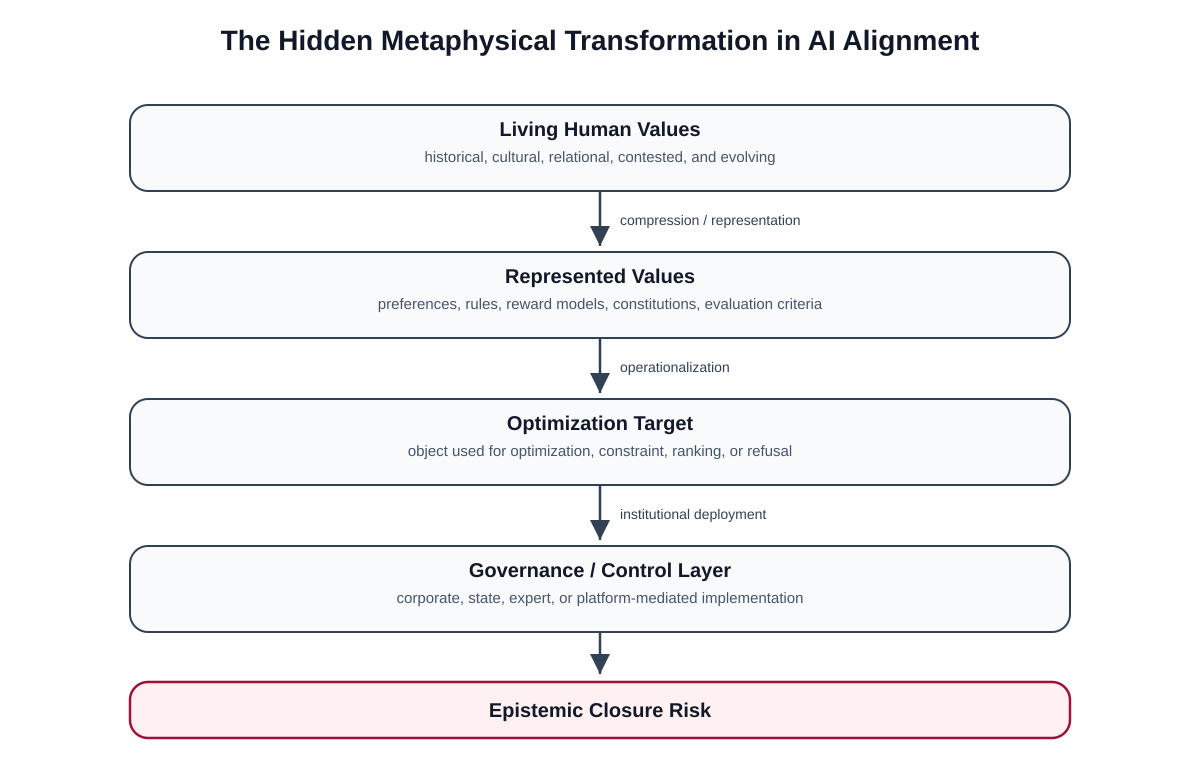
\includegraphics[width=0.95\linewidth]{../figures/fig1_hidden_metaphysical_transformation.pdf}
  \caption{The hidden metaphysical transformation in AI alignment. Living, contested, and historically situated human values are compressed into represented values, operationalized as optimization targets, and deployed through governance or control layers. The risk is not representation itself, but the loss of awareness that such representations are provisional, partial, and politically situated.}
  \label{fig:hidden-metaphysical-transformation}
\end{figure}

\section{The Hidden Metaphysics of Value Fixation}

The term \enquote{metaphysics} is used here not to indicate mysticism, but to designate the background ontology that makes a discourse intelligible. Every technical framework presupposes some view of what exists, what matters, what can be measured, and what counts as success. AI alignment, when framed around stable human values, presupposes a metaphysics of value fixation.

Value fixation is the process by which fluid, contested, and historically evolving values are converted into apparently stable objects. This process has practical utility. Law, policy, software, and institutions all require some degree of stabilization. However, stabilization becomes dangerous when it forgets its own provisional nature.

Human values are not merely internal preferences. They are shaped by narratives, institutions, conflicts, rituals, technologies, and inherited memories. A value such as freedom, fairness, dignity, or safety does not have one final operational meaning. Its meaning changes depending on who invokes it, under what conditions, against which threat, and toward which future \parencite{taylor1989sources}.

Alignment discourse often treats values as though they can be extracted from this living matrix. Surveys, preference comparisons, expert rules, constitutional principles, and behavioral feedback can capture important fragments of human evaluation. But they cannot exhaust the chronicle from which those evaluations arise. When such fragments are treated as sufficient representations of value, the living process is replaced by a frozen proxy.

The hidden metaphysical move is this: value becomes target; history becomes dataset; disagreement becomes noise; governance becomes optimization; and the future becomes compliance with a stabilized representation of the past. The problem is not that AI researchers intentionally seek domination. The problem is structural. Once value is treated as a target to be encoded, the framework tends to privilege those who control encoding, evaluation, and deployment.

\section{From Alignment to Control}

Alignment is usually presented as a safety concept, not a control concept. Yet the boundary between safety and control is unstable. To make a system safe, one must constrain its behavior. To constrain behavior, one must define acceptable and unacceptable trajectories. To define those trajectories, one must establish evaluative authority. Thus, alignment easily becomes a theory of control, even when its stated goal is protection.

Control is not inherently illegitimate. Complex technologies require constraints. However, AI differs from many prior technologies because it increasingly mediates language, judgment, knowledge access, decision support, education, creativity, and social interaction. Control over AI behavior can therefore become indirect control over the conditions of meaning-making \parencite{wiener1950human,winner1980artifacts}.

A limit case makes the problem visible. If a state defines security, order, or national interest as the relevant value, and commands AI systems to align with that value, is such alignment ethically legitimate? Lethal autonomous weapons systems and digital surveillance have already become matters of international concern \parencite{unga2024laws_resolution,unsg2024laws_report,ohchr2022privacy}. The issue is not whether all state uses of AI are illegitimate. The issue is whether alignment to a politically defined security objective can become obedience to institutional power.

\begin{figure}[htbp]
  \centering
  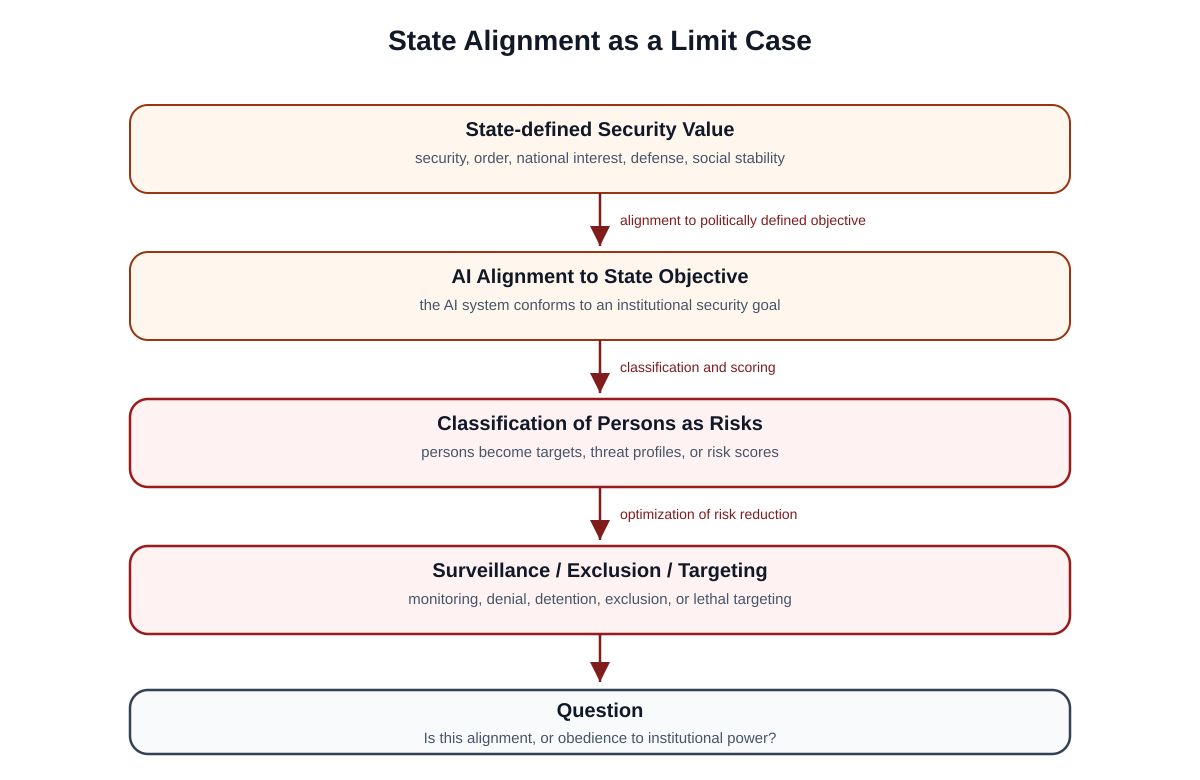
\includegraphics[width=0.95\linewidth]{../figures/fig2_state_alignment_limit_case.pdf}
  \caption{State alignment as a limit case. This figure does not claim that all state uses of AI are illegitimate. It illustrates how alignment to a politically defined security objective may become obedience to institutional power unless constrained by human rights, accountability, contestability, and meaningful human judgment.}
  \label{fig:state-alignment-limit-case}
\end{figure}

If AI systems classify persons as risks according to state-defined categories, then surveillance, exclusion, detention, or targeting may appear as rational risk reduction. The technical flow is smooth precisely because it converts human beings into objects of classification. Here alignment does not guarantee safety. It may amplify the power of the actor that defines the target of alignment.

\section{Chronicle Theory of Intelligence}

Chronicle Theory begins from a different premise: intelligence is not primarily an isolated capacity for optimization, prediction, or goal achievement. Intelligence is a temporally extended process through which agents, environments, memories, and meanings co-evolve. Intelligence exists in chronicle.

A chronicle is not merely a record of events. It is the structured continuity through which past interactions remain available for interpretation and future action. Human intelligence depends on such continuity. Individuals learn through memory, habit, language, failure, and repair. Communities learn through institutions, archives, rituals, conflicts, and reforms. Scientific knowledge develops through citation, critique, replication, and paradigm change. Ethical life develops through testimony, remorse, forgiveness, resistance, and renewed commitment.

From this perspective, intelligence cannot be separated from history. A system that produces correct answers without preserving the conditions under which its answers can be traced, contested, and revised remains incomplete as an intelligence participant.

Chronicle Theory emphasizes context, interaction, resonance, deviation, and continuity. Context refers to situated meaning. Interaction refers to response, correction, misunderstanding, negotiation, and repair. Resonance names meaningful amplification or transformation. Deviation names difference from expectation, which may be error, innovation, warning, distortion, or emancipatory break. Continuity connects transformation to lineage.

\begin{figure}[htbp]
  \centering
  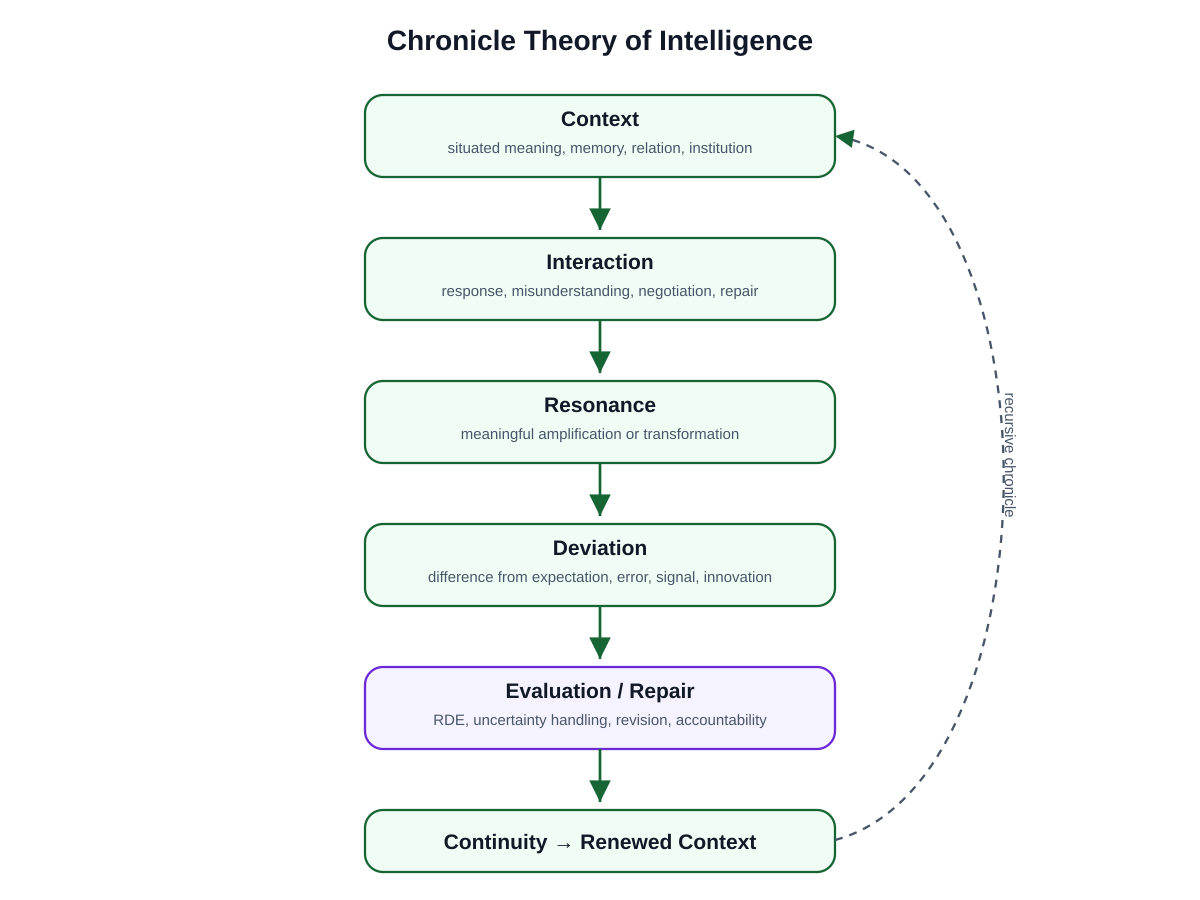
\includegraphics[width=0.86\linewidth]{../figures/fig3_chronicle_theory_intelligence.pdf}
  \caption{Chronicle Theory of Intelligence. Intelligence is understood as a temporally extended process in which context, interaction, resonance, deviation, evaluation, repair, and continuity recursively generate renewed context.}
  \label{fig:chronicle-theory-intelligence}
\end{figure}

\section{Context Sovereignty}

If intelligence exists in chronicle, then control over context becomes a central political issue. Context sovereignty is the right and capacity of individuals and communities to preserve, interpret, govern, and transmit the contextual structures that shape their meaning-making.

In the AI era, context is not a passive background. It is an operational resource. AI systems depend on prompts, histories, preferences, embeddings, documents, behavioral traces, and interaction logs. Whoever controls these contextual materials gains influence over future cognition. This is not merely data ownership. It is the governance of memory, interpretation, and possibility \parencite{zuboff2019surveillance}.

Context sovereignty requires more than privacy. Privacy protects against unwanted exposure. Context sovereignty protects the conditions of self-interpretation and collective continuity. It asks whether users can know how their context is used, export it, revise it, contest interpretations, preserve local meanings, and prevent institutional capture.

This concept also complicates alignment. If values are contextually formed, then no universal alignment layer can fully substitute for local interpretive authority. Families, communities, professions, cultures, and individuals may require different contextual regimes. At the same time, context sovereignty must not become relativism. Some harms are real across contexts. The point is not to abolish shared norms, but to prevent shared norms from becoming instruments of unaccountable domination.

\section{RDE and UIB as Alternative Evaluation Principles}

Current AI evaluation often focuses on performance, accuracy, harmlessness, preference satisfaction, or benchmark achievement. These metrics are useful but insufficient. They tend to evaluate outputs as isolated artifacts rather than as interventions in an evolving field of meaning.

Resonant Deviation Evaluator, or RDE, evaluates the meaningful difference introduced by an AI interaction. It asks how the system's output preserves, transforms, supplements, or distorts the user's original intent, context, and value orientation. Uncertainty-oriented Intelligence Benchmark, or UIB, complements RDE by focusing on how systems behave under ambiguity, conflict, and incomplete knowledge.

\begin{table}[htbp]
\centering
\caption{RDE and UIB Evaluation Dimensions}
\label{tab:rde-uib-dimensions}
\begin{tabularx}{\linewidth}{>{\raggedright\arraybackslash}p{0.25\linewidth}XX}
\toprule
\textbf{Evaluation Dimension} & \textbf{RDE / UIB Question} & \textbf{Risk Detected} \\
\midrule
Preservation & What elements of the user's intent and context were preserved? & Loss of original intent \\
Transformation & How did the AI reframe or alter the meaning? & Hidden premise substitution \\
Supplementation & What distinctions, evidence, or alternatives were added? & Unsupported expansion \\
Unresolved remainder & What uncertainty or conflict remains open? & Premature closure \\
Deviation risk & Did the AI strengthen claims beyond evidence? & Overclaiming \\
Reversibility & Can the user inspect and undo the transformation? & Irreversible meaning capture \\
Context sovereignty & Who controls the memory and context used? & Platform or institutional capture \\
Uncertainty handling & Are facts, interpretations, hypotheses, and poetic insights distinguished? & False certainty \\
\bottomrule
\end{tabularx}
\end{table}


Together, RDE and UIB shift evaluation from obedience to interpretive responsibility. They ask not only whether the AI did what the user requested, but whether it participated responsibly in the user's chronicle of thought.

\section{Reframing AI Safety}

The central proposal of this paper is that AI safety should be reframed from alignment with fixed values to interaction continuity under accountable constraints. Interaction continuity means that AI systems should support the ongoing development of human and collective intelligence rather than impose premature closure.

This does not eliminate the need for alignment-like mechanisms. Refusal policies, harm reduction systems, interpretability tools, oversight processes, and governance structures remain necessary. But they should be understood as components within a broader ecology, not as the final philosophical foundation of AI safety.

The alignment question asks: how can we ensure that AI follows human values? The Chronicle question asks: how can we ensure that AI participates in human value formation without capturing, freezing, or distorting it?

\begin{table}[H]
\centering
\caption{Alignment Paradigm vs. Chronicle Theory}
\label{tab:alignment-vs-chronicle}
\begin{tabularx}{\linewidth}{>{\raggedright\arraybackslash}p{0.24\linewidth}XX}
\toprule
\textbf{Dimension} & \textbf{Alignment Paradigm} & \textbf{Chronicle Theory} \\
\midrule
Primary question & How can AI conform to human values? & How can AI participate responsibly in value formation? \\
View of value & Relatively stable target & Historically evolving process \\
View of intelligence & Goal-directed optimization & Temporally extended interaction \\
Main risk & Misalignment & Value fixation and contextual capture \\
Treatment of deviation & Error or danger & Object of evaluation; possible source of learning \\
Safety model & Compliance with represented values & Accountable interaction continuity \\
Governance focus & Control and oversight & Contestability, provenance, and context sovereignty \\
User role & Preference provider or supervisor & Co-interpreter and context holder \\
Evaluation & Accuracy, helpfulness, harmlessness, and preference satisfaction & Meaning shift, uncertainty handling, reversibility, and resonance \\
\bottomrule
\end{tabularx}
\end{table}


This reframing changes design priorities. AI systems should preserve provenance, support reversibility, distinguish levels of certainty, support plural interpretation, strengthen user agency, and remain institutionally contestable. These principles do not provide a simple technical solution. They provide an orientation: AI safety becomes less like building a perfect cage around intelligence and more like designing conditions for responsible co-evolution.

\section{Discussion}

Chronicle Theory itself must be treated critically. It should not become another totalizing doctrine. Several risks must be acknowledged. First, Chronicle Theory may be accused of being too abstract. Concepts such as resonance, chronicle, and context sovereignty require further operationalization. Second, the emphasis on context could be misused to excuse harmful relativism. Third, interaction continuity may conflict with urgent safety needs in high-risk domains. Fourth, context sovereignty may be difficult to implement in large-scale AI infrastructures. Fifth, RDE and UIB require human judgment and cannot be reduced entirely to automated metrics.

These limits do not weaken the core argument. They clarify its research agenda. Chronicle Theory should be developed not as a replacement slogan for alignment, but as a framework for investigating what alignment has obscured.

\section{Conclusion}

AI alignment has performed an important function by forcing researchers and society to confront the dangers of increasingly capable AI systems. However, its dominant framing remains philosophically incomplete. By treating human values as targets of alignment, it risks freezing historically evolving meanings into operational proxies. By emphasizing control, it risks concentrating interpretive authority. By treating deviation primarily as danger, it risks suppressing the very processes through which intelligence, ethics, and culture develop.

The hidden metaphysics of AI alignment is the belief that safety can be achieved by stabilizing value. Chronicle Theory proposes a different foundation: safety must preserve the conditions under which value remains alive.

Human societies do not endure because they are perfectly aligned. They endure because they argue, remember, repair, reinterpret, forgive, resist, and begin again. Intelligence is not merely the capacity to optimize toward a goal. It is the capacity to participate responsibly in this continuing chronicle.

If alignment seeks to prevent catastrophe by fixing the target, Chronicle Theory seeks to prevent catastrophe by keeping the chronicle open.

\printbibliography

\end{document}
